%!TEX root = ./template-skripsi.tex
%-------------------------------------------------------------------------------
% 								BAB I
% 							LATAR BELAKANG
%-------------------------------------------------------------------------------

\chapter{PENDAHULUAN}

\section{Latar Belakang Masalah}

Mesin pencari atau \emph{search engine} adalah sebuah teknologi yang digunakan untuk mencari sebuah informasi yang tersedia di internet. Dengan memasukkan \emph{keyword} terkait hal yang ingin diketahui dan akan terlihat berbagai macam situs \emph{web} yang memiliki informasi sesuai. Perkembangan \emph{search engine} melahirkan penelitian yang berkelanjutan, meneliti bagaimana menciptakan algoritma yang efektif untuk menjalankan \emph{search engine} agar menampilkan pencarian yang relevan kepada pengguna.  

Penelitian \emph{search engine} yang dilakukan sebelumnya lebih terfokus untuk mengembangkan \emph{crawler} yang dapat berjalan secara \emph{multi-threaded} (\cite{fathan2021search}). Sedangkan pada penelitian selanjutnya mengarah pada \emph{refactoring crawler} dari penelitian sebelumnya dan mencari \emph{similarity score} dari setiap halaman situs \emph{web} yang di-\emph{crawling} (\cite{lazuardy2023search}). Dan penelitian lainnya saat melakukan pengumpulan data menggunakan \emph{crawler} yang sudah ada agar dapat dikelola dalam bentuk \emph{user interface} (\cite{aldian2024search}).

Kelemahan yang terdapat pada penelitian tersebut adalah \emph{crawling} hanya dapat berjalan pada satu perangkat saja. Hal itu dapat menghambat hasil dari \emph{crawling}, karena membutuhkan waktu lebih lama untuk mendapatkan hasil \emph{crawling} yang masif. Oleh karena itu, diperlukan cara agar \emph{crawler} dapat berjalan pada berbagai macam perangkat atau terdistribusi satu dengan lainnya. Serta kelemahan yang didapatkan bahwa proses \emph{crawling} dengan \emph{public IP address} dapat menyebabkan \emph{IP public} perangkat terblokir oleh Cloudflare atau layanan penyedia internet, sebab dianggap perilaku mencurigakan.

Terdapat juga kelemahan lainnya pada \emph{database}. \emph{Wasting storage} yang cukup besar terhadap kolom - kolom yang tidak terlalu diperlukan untuk \emph{similarity scoring}. Maka, peneliti melakukan analisis terkait \emph{database}-nya dengan melakukan \emph{crawling} selama 48 jam, didapatkan hasil laporan \emph{database} pada gambar 1.1. Total dari keseluruhan \emph{database}-nya adalah 8.7 GB.

\begin{figure}[H]
	\centering
	
\includegraphics[width=1\textwidth]{gambar/db_analisis}
	\caption{\emph{Analisis Database Penelitian Crawling}}
	\label{gambar:db_analisis}
\end{figure}

Terdapat \emph{wasting storage} pada \emph{table page\_list}, mengandung kumpulan \emph{tag} <li>. \emph{page\_scripts}, mengandung skrip \emph{javasript}. \emph{page\_styles}, mengandung \emph{style} dari CSS (\emph{Cascading Style Sheet}). \emph{page\_tables}, mengandung \emph{tag <table>}. Karena memiliki ukuran yang besar dan informasi yang didapatkan kurang berguna untuk melakukan \emph{page ranking}. Bahkan ukuran dari \emph{tables} yang disebutkan di atas dapat memenuhi setidaknya lebih dari 60\% dari total ukuran \emph{database}.

Sedangkan \emph{tables} yang berguna untuk hasil dari \emph{crawling} adalah: \emph{Table crawling}, untuk menjelaskan \emph{starting url}, \emph{total page}, durasi \emph{crawl}, dan tanggal \emph{crawling} berakhir. Lalu, pada \emph{table page\_linking} untuk mengetahui \emph{outgoing link}, yang nantinya akan digunakan untuk \emph{page ranking}. Pada \emph{table page\_information} diperlukan untuk mendapatkan \emph{initial page rank}, yang hasilnya didapatkan dari 1 / total baris \emph{table page\_information}. Dan juga berguna untuk \emph{document ranking tf-idf} dengan mengambil setiap kata yang ada. Melalui hasil analisis \emph{database} berikut, bahwa data penting yang digunakan untuk \emph{page rank} dan \emph{tf idf} adalah pada \emph{table crawling, page\_information, dan page\_linking}.

Diperlukan improvisasi pada algoritma dan menambahkan cara untuk membagi tugas \emph{crawling} supaya menjadi versi terdistribusi. \emph{Crawling} terdistribusi adalah melakukan \emph{crawling} secara terpisah ke setiap perangkat yang tersedia, guna membagi beban kerja dan dapat menghasilkan hasil \emph{crawler} dalam jumlah yang masif secara efisien serta efektif. Sebelum melakukan improvisasi \emph{crawler} yang sekarang menjadi terdistribusi, diperlukan pemahaman terkait sistem arsitekturnya.

Sistem arsitektur \emph{crawler} terdistribusi memiliki dua komponen penting, yaitu \emph{crawling system} dan \emph{crawling application}. \emph{Crawling System} meliputi \emph{crawl manager}, \emph{downloader}, dan \emph{DNS resolvers}. Sedangkan \emph{crawling application} yang melakukan proses \emph{crawling} yang berjalan pada perangkat.

% \begin{figure}[H]
% 	\centering
% 	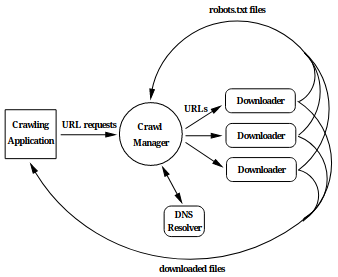
\includegraphics[width=0.5\textwidth]{gambar/arsitektur_terdistribusi}
% 	\caption{\emph{Arsitektur Sederhana Crawler Terdistribusi}}
% 	\label{gambar:arsitektur_terdistribusi}
% \end{figure}

Berdasarkan arsitektur sederhana didapatkan bahwa proses distribusi yang terjadi adalah pada sisi \emph{downloader}. Setelah \emph{crawl manager} melakukan \emph{crawling} pada suatu \emph{web} yang akan menghasilkan \emph{urls}, kemudian \emph{url} tersebut dilanjutkan kepada masing - masing \emph{downloader}. \emph{Downloader} ini terletak pada \emph{server} atau perangkat yang berbeda (\cite{shkapenyuk2002distributed}).

Komunikasi yang dilakukan dalam arsitektur tersebut dilakukan dalam dua cara yaitu, via \emph{socket} dan \emph{file system} untuk data yang lebih besar. Untuk improvisasi yang akan diterapkan dalam proyek ini akan lebih tertuju kepada penerapan \emph{socket}.

\emph{Socket} dapat dianggap sebagai \emph{endpoint} dalam \emph{two-way communication channel}. \emph{Socket} dapat melakukan komunikasi antara dua proses, baik dalam satu perangkat atau perangkat yang berbeda. Untuk dapat melakukan komunikasi dua arah, terlebih dahulu dipahami arsitektur \emph{client-server}. \emph{Client} dapat berupa PC, laptop, telepon seluler, dll. Dan setiap \emph{client} memiliki IP \emph{address}-nya masing - masing. Untuk dapat melakukan komunikasi atau pertukaran data diperlukan setiap \emph{client} untuk terhubung ke sebuah \emph{server}. \emph{Server} pun juga memiliki IP \emph{address}. Agar \emph{client} dapat terhubung ke \emph{server}, maka ia harus mengetahui IP \emph{server}. Dan setiap \emph{client} yang terhubung ke \emph{server} akan dapat berkomunikasi via \emph{server} dalam hal ini akan menggunakan \emph{socket} (\cite{ibm2021whatissocket}).

% Penggunaan SOCK\_STREAM berarti memakai \emph{protocol} TCP. Kalau ingin memakai \emph{protocol} UDP, maka menggunakan SOCK\_DGRAM. Di sini saya menggunakan TCP karena beberapa keunggulan seperti, \emph{reliable} (dapat mendeteksi \emph{packet loss}), dapat memastikan data terkirim, \emph{sequential} (data yang dikirim berurutan), \emph{byte stream} (data yang dikirim dalam bentuk \emph{byte}, lebih efisien), \emph{keeps up connection}. Kalau dibandingkan dengan UDP seperti, \emph{sends one datagram, no order and guarantee, more realtime} (karena tidak memperdulikan \emph{packet loss}, jadi lebih cepat), \emph{less network} and \emph{pc stress} \cite{neuralnine2021socket}.

% \begin{figure}[H]
% 	\centering
% 	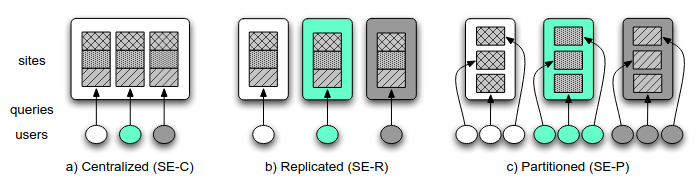
\includegraphics[width=0.85\textwidth]{gambar/arsitektur_query_processing}
% 	\caption{\emph{Arsitektur Sederhana Crawler Terdistribusi}}
% 	\label{gambar:arsitektur_query_processing}
% \end{figure}

Pada penelitian lain terkait \emph{query processing} dan alokasi komputasional \emph{crawler} terdistribusi yang dilakukan oleh Cambazoglu terdapat beberapa jenis arsitektur berdasarkan cara penyimpanan \emph{index}-nya. Secara \emph{centralized} (SE-C), \emph{replicated} (SE-R), dan \emph{partitioned} (SE-P). Ada juga arsitektur gabungan antara \emph{partial replication} dan \emph{query forwarding} (SE-H). Arsitektur \emph{centralized} masih banyak digunakan sampai sekarang, apalagi dalam skala yang lebih kecil (\cite{cambazoglu2009quantifying}).

% \begin{figure}[H]
% 	\centering
% 	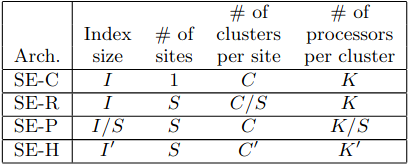
\includegraphics[width=0.5\textwidth]{gambar/resource_allocation_on_search_engine}
% 	\caption{\emph{Alokasi Sumber Daya pada Berbagai Arsitektur Search Engine}}
% 	\label{gambar:resource_allocation_on_search_engine}
% \end{figure}

% Pada pemrosesan query ada dua tipe cost, fixed cost independent dari jumlah processor dan cost linear dengan pertambahan jumlah processor. Rata - rata waktu yang diperlukan untuk memproses query (T) dapat direpresentasikan dalam persamaan 

% \begin{equation*}
%   T = a + b × Iavg/K,
% \end{equation*}
% a adalah fixed time cost, b adalah time cost untuk memproses byte pada inverted list, Iavg adalah rata - rata ukuran index. dan K adalah jumlah processor di tiap klaster \cite{cambazoglu2009quantifying}.

% \begin{figure}[H]
% 	\centering
% 	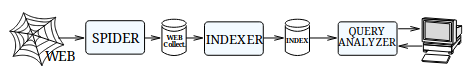
\includegraphics[width=0.85\textwidth]{gambar/typical_web_search_engine_architecture}
% 	\caption{\emph{Tipikal Arsitektur Web Search Engine}}
% 	\label{gambar:typical_web_search_engine_architecture}
% \end{figure}

Pada penelitian yang dilakukan oleh (\cite{orlando2002design}) menjelaskan bahwa dalam \emph{web search engine} terdiri dari \emph{spidering system}. Kesatuan dari sistem ini berjalan secara paralel, yang mana \emph{crawler} akan mengunjungi setiap \emph{web} dan mengumpulkan informasi yang diperlukan. Inti utama dalam \emph{Information Retrieval} (IR) adalah \emph{indexer} dan \emph{query analyzer}. 

% Hasil dari informasi yang didapatkan akan di-\emph{ranking} berdasarkan kesesuaiannya dengan \emph{query} yang dimasukkan, untuk mendapatkan hasil akhir yang sesuai dan efisien, banyak arsitektur search engine sekarang menerapkan Inverted List untuk indexing. Ada dua komponen penting dari Inverted List yaitu Lexicon dan Postings list.

Pada tahapan \emph{query analyzer} melakukan proses paralel terhadap \emph{Query Brokers} dan \emph{Local Searchers}. Dilakukan secara terdistribusi menggunakan teknik \emph{document partitioning}. Strategi untuk membuat paralel \emph{web search engine} harus memenuhi dua hal, \emph{task parallel} dan \emph{data parallel}. Untuk menghindari eksploitasi \emph{processor} secara berlebihan, maka diperlukan \emph{load balancer}, agar setiap \emph{query} dapat berjalan secara efisien dan efektif. Dengan melakukan pembagian \emph{task} secara paralel. Oleh karena setiap \emph{query} diproses secara terpisah, maka juga memiliki partisi \emph{database}-nya tersendiri. Untuk itu diperlukan kombinasi antara \emph{task} dan \emph{data parallel}, agar hasil akhir dari proses \emph{search engine} lebih relevan (\cite{orlando2002design}).

Pada penelitian lain dijelaskan juga mengenai distribusi algoritma, walaupun diterapkan pada perhitungan \emph{page rank} agar lebih efisien memori dalam melakukan perhitungan. Karena untuk perhitungannya diperlukan memori yang besar. Oleh karena itu, diperlukan proses efisiensi memori (\cite{farhan2023page}). Walaupun begitu data perhitungan akan berkurang karena efisiensi memori, memang ada hal yang menjadi timbal baliknya. Nanti hasil dari penelitian tersebut juga akan diterapkan untuk penelitian lebih lanjut setelah penelitian yang penulis lakukan.

Berdasarkan beberapa rujukan sebelumnya, hasil dari penelitian ini adalah sebuah \emph{crawler} yang berjalan secara terdistribusi yang akan mengimplementasikan penggunaan \emph{socket} dalam mendistribusikan tugas ke setiap perangkat, serta peningkatan jumlah data yang terkumpul.

% Menerapkan \emph{time cost efficiency} dalam melakukan \emph{query processing}, serta melakukan \emph{task parallel} yang baik dengan keseimbangan tugas. Untuk arsitekturnya akan merujuk arsitektur gabungan antara \emph{partial replication} dan \emph{query forwarding} (SE-H).

\section{Rumusan Masalah}
Berdasarkan uraian pada latar belakang yang diutarakan di atas, maka perumusan masalah pada penelitian ini adalah "\textbf{bagaimana meningkatkan efisien \emph{crawling} dengan cara terdistribusi?}".

\section{Pembatasan Masalah}
Pembatasan masalah pada penelitian ini antara lain:
\begin{enumerate}
	\item Pengembangan arsitektur \emph{crawler} menjadi versi terdistribusi dengan skala kinerja 2 hingga 5 perangkat.
	\item \emph{Crawler} terdistribusi yang dikembangkan menggunakan \emph{socket} sebagai media komunikasi antar perangkat.
	\item Pengujian terhadap \emph{crawler} terdistribusi dan tidak terdistribusi yang akan mempertimbangkan faktor-faktor seperti kecepatan crawling dan efisiensi penggunaan sumber daya.
\end{enumerate}

\section{Tujuan Penelitian}
Tujuan penelitian pada penelitian ini antara lain:
\begin{enumerate}
	\item Mengembangkan arsitektur \emph{distributed crawler}.
	\item Membuat implementasi \emph{socket} untuk memenuhi kebutuhan improvisasi \emph{crawler}.
\end{enumerate}

\section{Manfaat Penelitian}
\begin{enumerate}
	\item Bagi penulis
		
	Menambah pengetahuan di bidang sistem terdistribusi mengenai \emph{search engine} dan \emph{crawling}, mengasah kemampuan programming, dan memperoleh gelar sarjana di bidang Ilmu Komputer. Selain itu, penulisan ini juga merupakan media bagi penulis untuk mengaplikasikan ilmu yang didapat di kampus ke kehidupan masyarakat.
		
	\item Bagi Universitas Negeri Jakarta 
	 	
	Menjadi pertimbangan dan evaluasi akademik khususnya Program Studi Ilmu Komputer dalam penyusunan skripsi sehingga dapat meningkatkan kualitas akademik di program studi Ilmu Komputer Universitas Negeri Jakarta serta meningkatkan kualitas lulusannya.
	 			
\end{enumerate}


% Baris ini digunakan untuk membantu dalam melakukan sitasi
% Karena diapit dengan comment, maka baris ini akan diabaikan
% oleh compiler LaTeX.
\begin{comment}
\bibliography{daftar-pustaka}
\end{comment}
